\pdfoutput=1
 
\documentclass{l4proj}
\usepackage[usenames,dvipsnames]{xcolor}
\usepackage{enumitem}
\usepackage{hyperref}
\usepackage{titlesec}
\usepackage{listings}
\titlespacing{\subsubsection}{0pt}{6pt}{6pt}
\definecolor{properBlue}{HTML}{336699}
\hypersetup{
    colorlinks,
    citecolor=properBlue,
    filecolor=properBlue,
    linkcolor=properBlue,
    urlcolor=properBlue
}
 
\begin{document}
\title{Package Recommendation Engine}
\author{Keir Alexander Smith}
\date{March 15, 2015}
\maketitle
 
\begin{abstract}
This paper covers the construction of a basic recommendation engine for operating system packages, specifically for use with the DNF package manager. The tool should allow users to discover useful packages through an easy to use command line interface.
\end{abstract}
 
%\educationalconsent
\tableofcontents

\lstset{ %
language=Python,              % choose the language of the code
basicstyle=\scriptsize,     % the size of the fonts that are used for the code
%basicstyle=\tiny,     % the size of the fonts that are used for the code
numbers=left,               % where to put the line-numbers
%numberstyle=\tiny,    % the size of the fonts that are used for the line-numbers
numberstyle=\scriptsize,    % the size of the fonts that are used for the line-numbers
numbersep=10pt,             % how far the line-numbers are from the code
frame=trBL,                 % adds a frame around the code
%tabsize=2,                  % sets default tabsize to 2 spaces
captionpos=b,               % sets the caption-position to bottom
breaklines=true,            % sets automatic line breaking
breakatwhitespace=false,    % sets if automatic breaks should only happen at whitespace
showstringspaces=false,     % Don't show underscores as space characters
frameround=fttt
}
 
%%%%%%%%%%%%%%%%%%
%                %
%  INTRODUCTION  %
%                %
%%%%%%%%%%%%%%%%%%
 
\chapter{Introduction}
\pagenumbering{arabic}
 
\section{Problem overview}
In a modern operating system there exists many packages for end users to install and this collection grows every day. Finding useful packages to install can be a laborious task, often involving the use of the internet to track down the package the user has been looking for, if it exists.\\
Furthermore there exists little support for installing packages commonly installed side by side. For example a user who has vim installed also installs Java Development Kit (JDK), the user may not be aware of the existence of a Java plugin for vim which is extremely useful.

\section{Motivation}
Package management is an interesting and very useful tool for many users, however the basic implementation has been static for many years. With the addition of this tool, we could see a decrease in users having to use search engines to look for packages they should be able to discover easily on command line. 
 
\section{Aims}
This project aims to attempt to address the issues discussed above. Fore-mostly the problem of finding new packages by offering a powerful recommendation system for users to discover packages.\\
Consider a user on a Linux machine, looking for any new useful developer tools to help their work flow. Using an internet search engine returns a fairly miss match set of results, this project aims to supply that user with a command line interface where they can ask for a recommendation based on package of their choice. In this case our user asks for a recommendation based off of the JDK and is returned with a list of useful debugging tools and plugins which they weren't aware of.

\section{Report outline}
This report will begin by looking at the research undertaken at the outset of the project, then continue into design of the system. This will lead into the implementation and finally the evaluation and conclusion.
 
%%%%%%%%%%%%%%%%
%              %
%  BACKGROUND  %
%              %
%%%%%%%%%%%%%%%%
 
\chapter{Background}
A package manager allows users to search for, install and update packages containing useful programs. For many years Unix has relied on package managers to allow easy management of tools and underlying applications. However in recent times, as package numbers increase and the ease of search engines becomes more prominent, searching using a command line tool has become less prevalent. Unless a user knows exactly what they want, often times they will resort to a internet search engine to find new packages.\\

\section{Modern Graphical Package Managers}
A more modern solution to this problem is the use of Graphical User Interfaces (GUIs) to abstract the annoyance of searching on command line away from the user. However this requires that the user is running a system with graphical output, a luxury which is often not found when running Virtual Machines (VMs) or using Secure Shell (SSH).\\

\section{NUGET Concierge}
In a similar vein NUGET (a .NET package manager) experimented with recommendations based off the same method this project uses, with weighting between packages rather than between user's install habits. A user could upload their project's meta data and Concierge would list packages the user may be interested in using based of what their project needs.\\

\section{DNF}
This project aims to supply similar functionality to users of DNF, Fedora 21's new package manager. DNF allows plugins to be easily added by simply dropping a Python file into the plugins directory. This allows DNF to be extended easily with little hardship from the user. Building this functionality into DNF is exactly the behaviour this project aims to provide to the end user.\\ 

%%%%%%%%%%%%
%          %
%  DESIGN  %
%          %
%%%%%%%%%%%%
 
\chapter{Design}
This system comes in two parts, a client side plugin for DNF which the user installs by dropping a single Python script into the correct directory. Also a graph server side database to store user's installed packages anonymously and provide data for recommendations.\\
Each of these components will be discussed in their own sections.

\section{Recommend Plugin}
In the choice between DNF and dpkg/apt, DNF was chosen due to it's excellent plugin support over the alternative.\\
The Recommend plugin has two key features:
\begin{itemize}
\item Request recommendation from server
\item Upload user's installed packages anonymously
\end{itemize}
Both functions require a connection to the back end database, a connection over the internet is assumed.\\
The plugin needed to be easy to use, to counter the desire to open a browser. With this in mind it is designed with two clear commands.\\
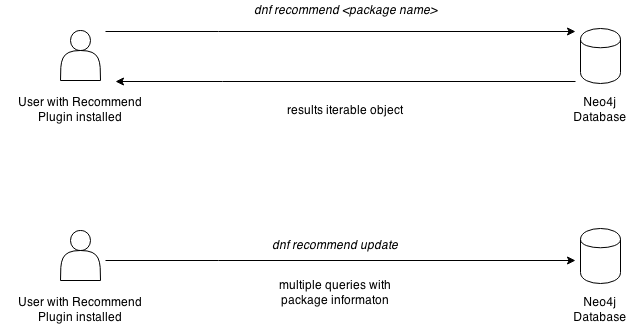
\includegraphics[scale=0.75]{images/recommend_api.png}


\section{Database}
The project requires a back end data storage median. Immediately a database comes to mind for a long term, concurrent access method of storing and returning large volumes of data. Below the various potential choices of database are discussed.

\subsection{Selection}
Neo4j was selected as the database of choice for this project. There are several key reasons for this:
\begin{itemize}
\item NOSQL database which is built for finding paths in mind
\item A standard SQL database would make storing the data complex
\item Neo4j is built to scale across distributed systems being a modern database solution
\end{itemize}

\subsection{Internal Structure}
Internally the structure of the graph can be seen in the figure below.
\vspace{10 px}\\
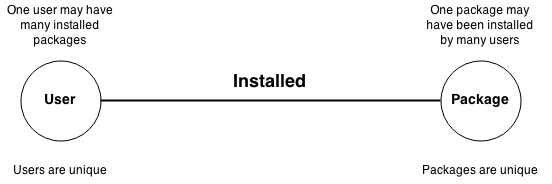
\includegraphics[scale=0.9]{images/recommend_graph.png}

 
%%%%%%%%%%%%%%%%%%%%
%                  %
%  IMPLEMENTATION  %
%                  %
%%%%%%%%%%%%%%%%%%%%
 
\chapter{Implementation}
In regards to development environment, all work took place using a GitHub repository with all the Python scripts kept up to date there. Locally the Recommend plugin was kept in the Git repository folder which was then sym linked to the DNF plugin folder. This enabled work and change tracking to take place without disturbing work flow to test the plugin.\\
With the design settled, work began with a 'Wizard of Oz' style mock up, where the user could use the command line interface as if the system were complete, however anything they go back was simply place holder.

\section{First Pass Mock UI}
For this initial development two features needed to be implemented. A command to push installed packages to server and request a recommendation from the server.\\
DNF allows a developer to hook into its core functionality by extending classes, which allows new commands to be written and functionality added in a single Python script. Figure 4.1 and 4.2 shows two classes extending DNF plugin and command classes respectively.
\begin{figure}
\lstset{caption={Recommend Class},label=codeRecClass}
\lstinputlisting[firstline=15, lastline=37]{code/recommend.py}
\end{figure}
\begin{figure}
\lstset{caption={Recommend Command Class},label=codeRecCommClass}
\lstinputlisting[firstline=53]{code/recommend.py}
\end{figure}

\section{Testing}
In order to test this system, two scripts were written in Python to fill the database with both real and mock data. Several small Cypher scripts were also written to test that the database was working internally.\\
Listing 4.3 and 4.4 show the Python scripts for entering data.\\
\begin{figure}
\lstset{caption={Fills the graph with real data},label=codeGraphReal}
\lstinputlisting{code/graph.py}
\end{figure}
\begin{figure}
\lstset{caption={Fills the graph with mock data},label=codeGraphMock}
\lstinputlisting{code/graph_filler.py}
\end{figure}

\section{Back End Implementation}
Now that some form of client side had been written, the back end could be implemented. This turned into a simple case of downloading and running a Neo4j instance on a local machine to test scripts.\\
The initial script written, shown in figure, read a list of packages from a text file in the format which DNF dumps them and then created each on the database and tied them to a user with a fake ID.\\
With that was in place, scripts to find sets of recommendations between packages can be written and tested.

\section{Bringing it together}
With the client side UI already written and tested, it was a simple case of changing a constant defining the server address to the operational database which was running on local host.
 
%%%%%%%%%%%%%%%%
%              %
%  EVALUATION  %
%              %
%%%%%%%%%%%%%%%%
 
\chapter{Evaluation}
%or lack thereof
\section{Survey Response}
 
%%%%%%%%%%%%%%%%
%              %
%  CONCLUSION  %
%              %
%%%%%%%%%%%%%%%%
 
\chapter{Conclusion}

\section{Summary}
%Lets talk about how kinda rubbish it really is unless its making some really interesting recommendations
\section{Future Work}
There exists a lot of scope for this project to expand. This report will discuss two interesting areas for potential future work.

\subsection{Package Groups}
As a potential future addition, commonly installed package groups could be identified on the back end, which would be pushed forward to end users, allowing them to quickly install a complete set of tools.\\
An example of this would be web developers, who commonly install at least the three main browsers\footnote{Google Chrome, Mozilla Firefox and Safari} and any debugging/developer tools associated with them.\footnote{For example Firebug}\\
This kind of powerful inferencing can be done using a graph database made to look for groups like this. If it's possible to then analyse the group and identify what it is, this would give users a lot of power when installing packages.  

\subsection{Weighted Relationships} 
Weighted relationships is something which NUGET Concierge used to make its recommendations. It's a one directional value assigned between two package nodes to determine how likely it is that one is installed on the same system with the other.\\
At it's core, it's very simple, however we could go lengths to make this weighting more meaningful, perhaps through the use of labels or special cases we can identify when best to include packages in a recommendation. For example it may be the case that package X is usually only installed when package Y is installed and Z isn't. A weighted relationship would not identify this as it would only recommend the most common. By tagging the relationships we can ensure the correct recommendation is made to the user.

\section{Lessons Learned}
%Start your dissertation earlier
%%%%%%%%%%%%%%%%
%              %
%  APPENDICES  %
%              %
%%%%%%%%%%%%%%%%
 
\begin{appendices}
 
\chapter{Name of the first appendix}
 
\end{appendices}
 
%%%%%%%%%%%%%%%%%%%
%                 %
%  BIBLIOGRAPHY   %
%                 %
%%%%%%%%%%%%%%%%%%%
 
\bibliographystyle{plain}
\bibliography{bib}
\end{document}